In the following diagrams, the component interfaces are presented and the dependencies between the parts of the application server are shown. Each Interfaces which is already explained in the runtime view are detailed here with all the functions and methods they include. Like the component diagram, has three parts to implement three services in the same manner this has three separate diagram to explain all the interfaces and there interactions.
\begin{figure}[H]
	\begin{center}
		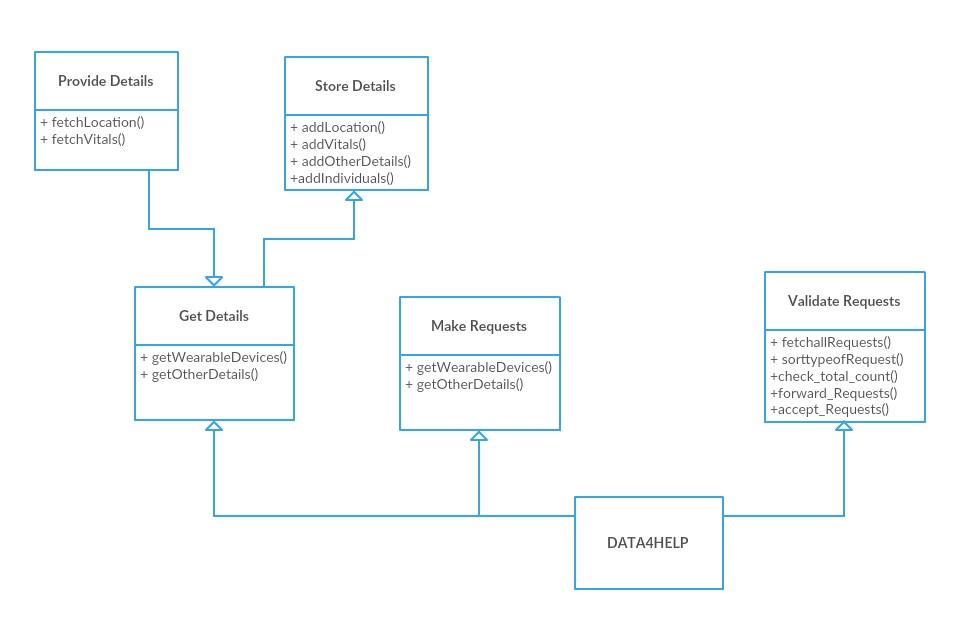
\includegraphics[width=\textwidth]{./DD_Diagrams/InterfaceData4Help.jpg}
      \caption{Component Interface Diagram for Data4Help}
        \label{TrackMe_int1}
	\end{center}
\end{figure}
\begin{figure}[H]
	\begin{center}
		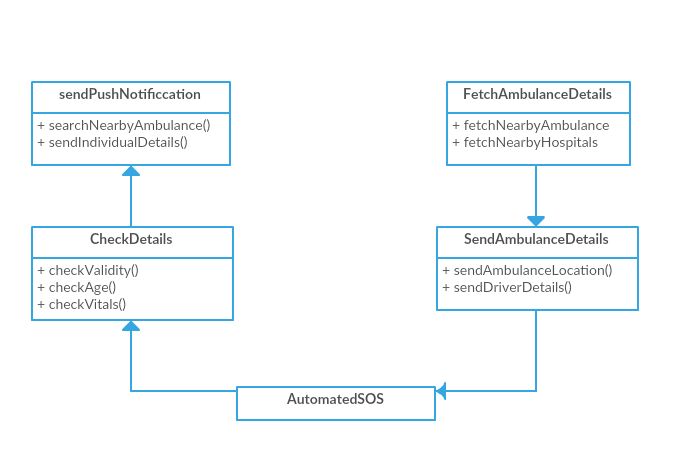
\includegraphics[width=\textwidth]{./DD_Diagrams/InterfaceAutomatedSOS.png}
      \caption{Component Interface Diagram for AutomatedSOS}
        \label{TrackMe_int2}
	\end{center}
\end{figure}
\begin{figure}[H]
	\begin{center}
		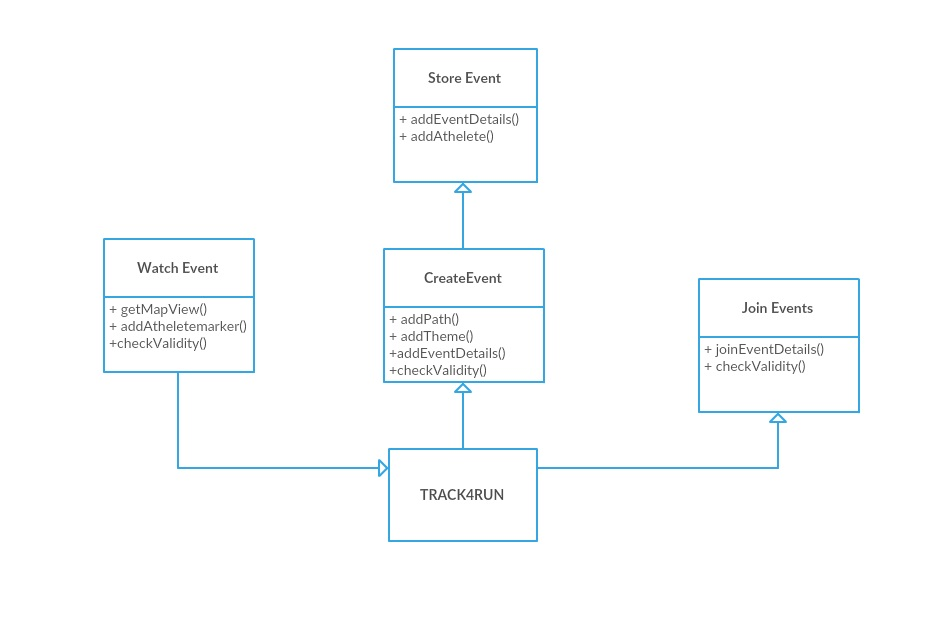
\includegraphics[width=\textwidth]{./DD_Diagrams/InterfaceTrack4Run.jpg}
      \caption{Component Interface Diagram for Track4Run}
        \label{TrackMe_int3}
	\end{center}
\end{figure}